\chapter{Selective sweeps on different pigmentation genes mediate convergent evolution of island melanism in two incipient bird species} \label{chapter3}

\textit{Content of this chapter was published in PLoS Genetics (2022) under the title ``Selective sweeps on different pigmentation genes mediate convergent evolution of island melanism in two incipient bird species" by Leonardo Campagna, Ziyi Mo, Adam Siepel and J. Albert C. Uy. L.C. conceptualized the study, curated data, performed formal analyses, developed methodology and wrote the manuscript. Z.M. characterized selective sweeps in the bird populations using the SIA method, developed methodology and edited the manuscript. A.S. developed methodology and edited the manuscript. J.A.C.U. conceptualized the study, curated data, performed formal analyses, developed methodology and wrote the manuscript.}

\section{Abstract}

Insular organisms often evolve predictable phenotypes, like flightlessness, extreme body sizes, or increased melanin deposition. The evolutionary forces and molecular targets mediating these patterns remain mostly unknown. Here we study the Chestnut-bellied Monarch (\textit{Monarcha castaneiventris}) from the Solomon Islands, a complex of closely related subspecies in the early stages of speciation. On the large island of Makira \textit{M. c. megarhynchus} has a chestnut belly, whereas on the small satellite islands of Ugi, and \ac{SA/SC} \textit{M. c. ugiensis} is entirely iridescent blue-black (i.e., melanic). Melanism has likely evolved twice, as the Ugi and \ac{SA/SC} populations were established independently. To investigate the genetic basis of melanism on each island we generated whole genome sequence data from all three populations. Non-synonymous mutations at the \textit{MC1R} pigmentation gene are associated with melanism on \ac{SA/SC}, while \textit{ASIP}, an antagonistic ligand of \textit{MC1R}, is associated with melanism on Ugi. Both genes show evidence of selective sweeps in traditional summary statistics and statistics derived from the \acf{ARG}. Using the \ac{ARG} in combination with machine learning, we inferred selection strength, timing of onset and allele frequency trajectories. \textit{MC1R} shows evidence of a recent, strong, soft selective sweep. The region including \textit{ASIP} shows more complex signatures; however, we find evidence for sweeps in mutations near \textit{ASIP}, which are comparatively older than those on \textit{MC1R} and have been under relatively strong selection. Overall, our study shows convergent melanism results from selective sweeps at independent molecular targets, evolving in taxa where coloration likely mediates reproductive isolation with the neighboring chestnut-bellied subspecies.

\section{Introduction}
The extent to which evolutionary change can be predicted has been a longstanding matter of debate in evolutionary biology (\cite{gould1989wonderful,blount2018contingency,grant2002unpredictable}). Instances of convergent evolution support the argument that evolutionary change can be deterministic, yet stochastic historical events can lead to divergent outcomes from recently split taxa. A better understanding of the eco-evolutionary forces and genetic mechanisms behind evolutionary changes will shed light on the conditions under which deterministic or stochastic outcomes can occur. Some examples of convergent evolution occurred deep in the tree of life, like the independent origins of wings in birds, bats and insects (\cite{blount2018contingency}), while other cases represent more recent (and potentially ongoing) phenomena like the repeated radiations of ecomorphs in Caribbean lizards (\cite{mahler2013exceptional}), the loss of flight associated to insularity in insects and birds (\cite{roff1994evolution,wright2016predictable}) or the evolution of island melanism (\cite{mundy2005window}). These recent classic examples of phenotypic convergence can be leveraged to study the evolutionary forces and molecular mechanisms behind phenotypic change. Here we focus on island melanism in birds, a phenotype that involves the increased deposition of eumelanin, which leads to entirely black plumage coloration (\cite{theron2001molecular,uy2016mutations,walsh2021patterns}).

The Chestnut-bellied Monarch (\textit{Monarcha castaneiventris}) from the Solomon Islands represents a complex of closely related subspecies which are in the early stages of speciation and vary in plumage color, song, and body size (\cite{mayr1999systematics,mayr2001birds,uy2009plumage}). One of these subspecies, \textit{M. c. ugiensis}, has entirely iridescent blue-black plumage, and is found on the small satellite islands to the north and southeast of the larger island of Makira (Fig. \ref{fig:mon-F1}A). In contrast, the endemic subspecies on Makira is \textit{M. c. megarhynchus} and has a chestnut belly and iridescent blue-black upper parts. Phylogenetic analyses using reduced-representation genomic data show that \textit{M. c. ugiensis} individuals from the satellite islands of Ugi, and \acf{SA/SC} are independently derived from the chestnut-bellied Makira population, suggesting that \textit{M. c. ugiensis} is polyphyletic and melanism has evolved repeatedly and convergently (\cite{cooper2017genomic}). A candidate gene study suggested that the molecular basis of increased melanin deposition differs between the Ugi and \ac{SA/SC} populations (\cite{uy2016mutations}). Melanism on each of the satellite islands is associated with mutations that affect the coding sequence of the \textit{MC1R}/\textit{ASIP} receptor and ligand pair, two molecules that regulate the balance between the production of eumelanin (a pigment conferring black/gray coloration) and pheomelanin (a pigment which leads to brown/yellow coloration). While the melanic individuals from \ac{SA/SC} carry a derived non-synonymous mutation on the \textit{MC1R} receptor, their counterparts from Ugi possess a non-synonymous mutation on the \textit{ASIP} ligand, and heterozygotes at either mutation display an intermediate coloration phenotype (Fig. \ref{fig:mon-F1}B; \cite{uy2016mutations}). Finally, it is likely that changes in plumage color mediated by these mutations generate prezygotic reproductive isolation between the melanic populations on the satellite islands and the chestnut-bellied population on nearby Makira, as territorial males discriminate individuals by their phenotype, and respond predominantly to simulated territorial intrusions of males with the local plumage (and song) traits (\cite{uy2009difference,uy2013variation}). Convergent melanism, therefore, may result in repeated speciation between the chestnut-bellied population of Makira, and each of the two melanic populations of Ugi and \ac{SA/SC}.

\begin{figure}
    \centering
    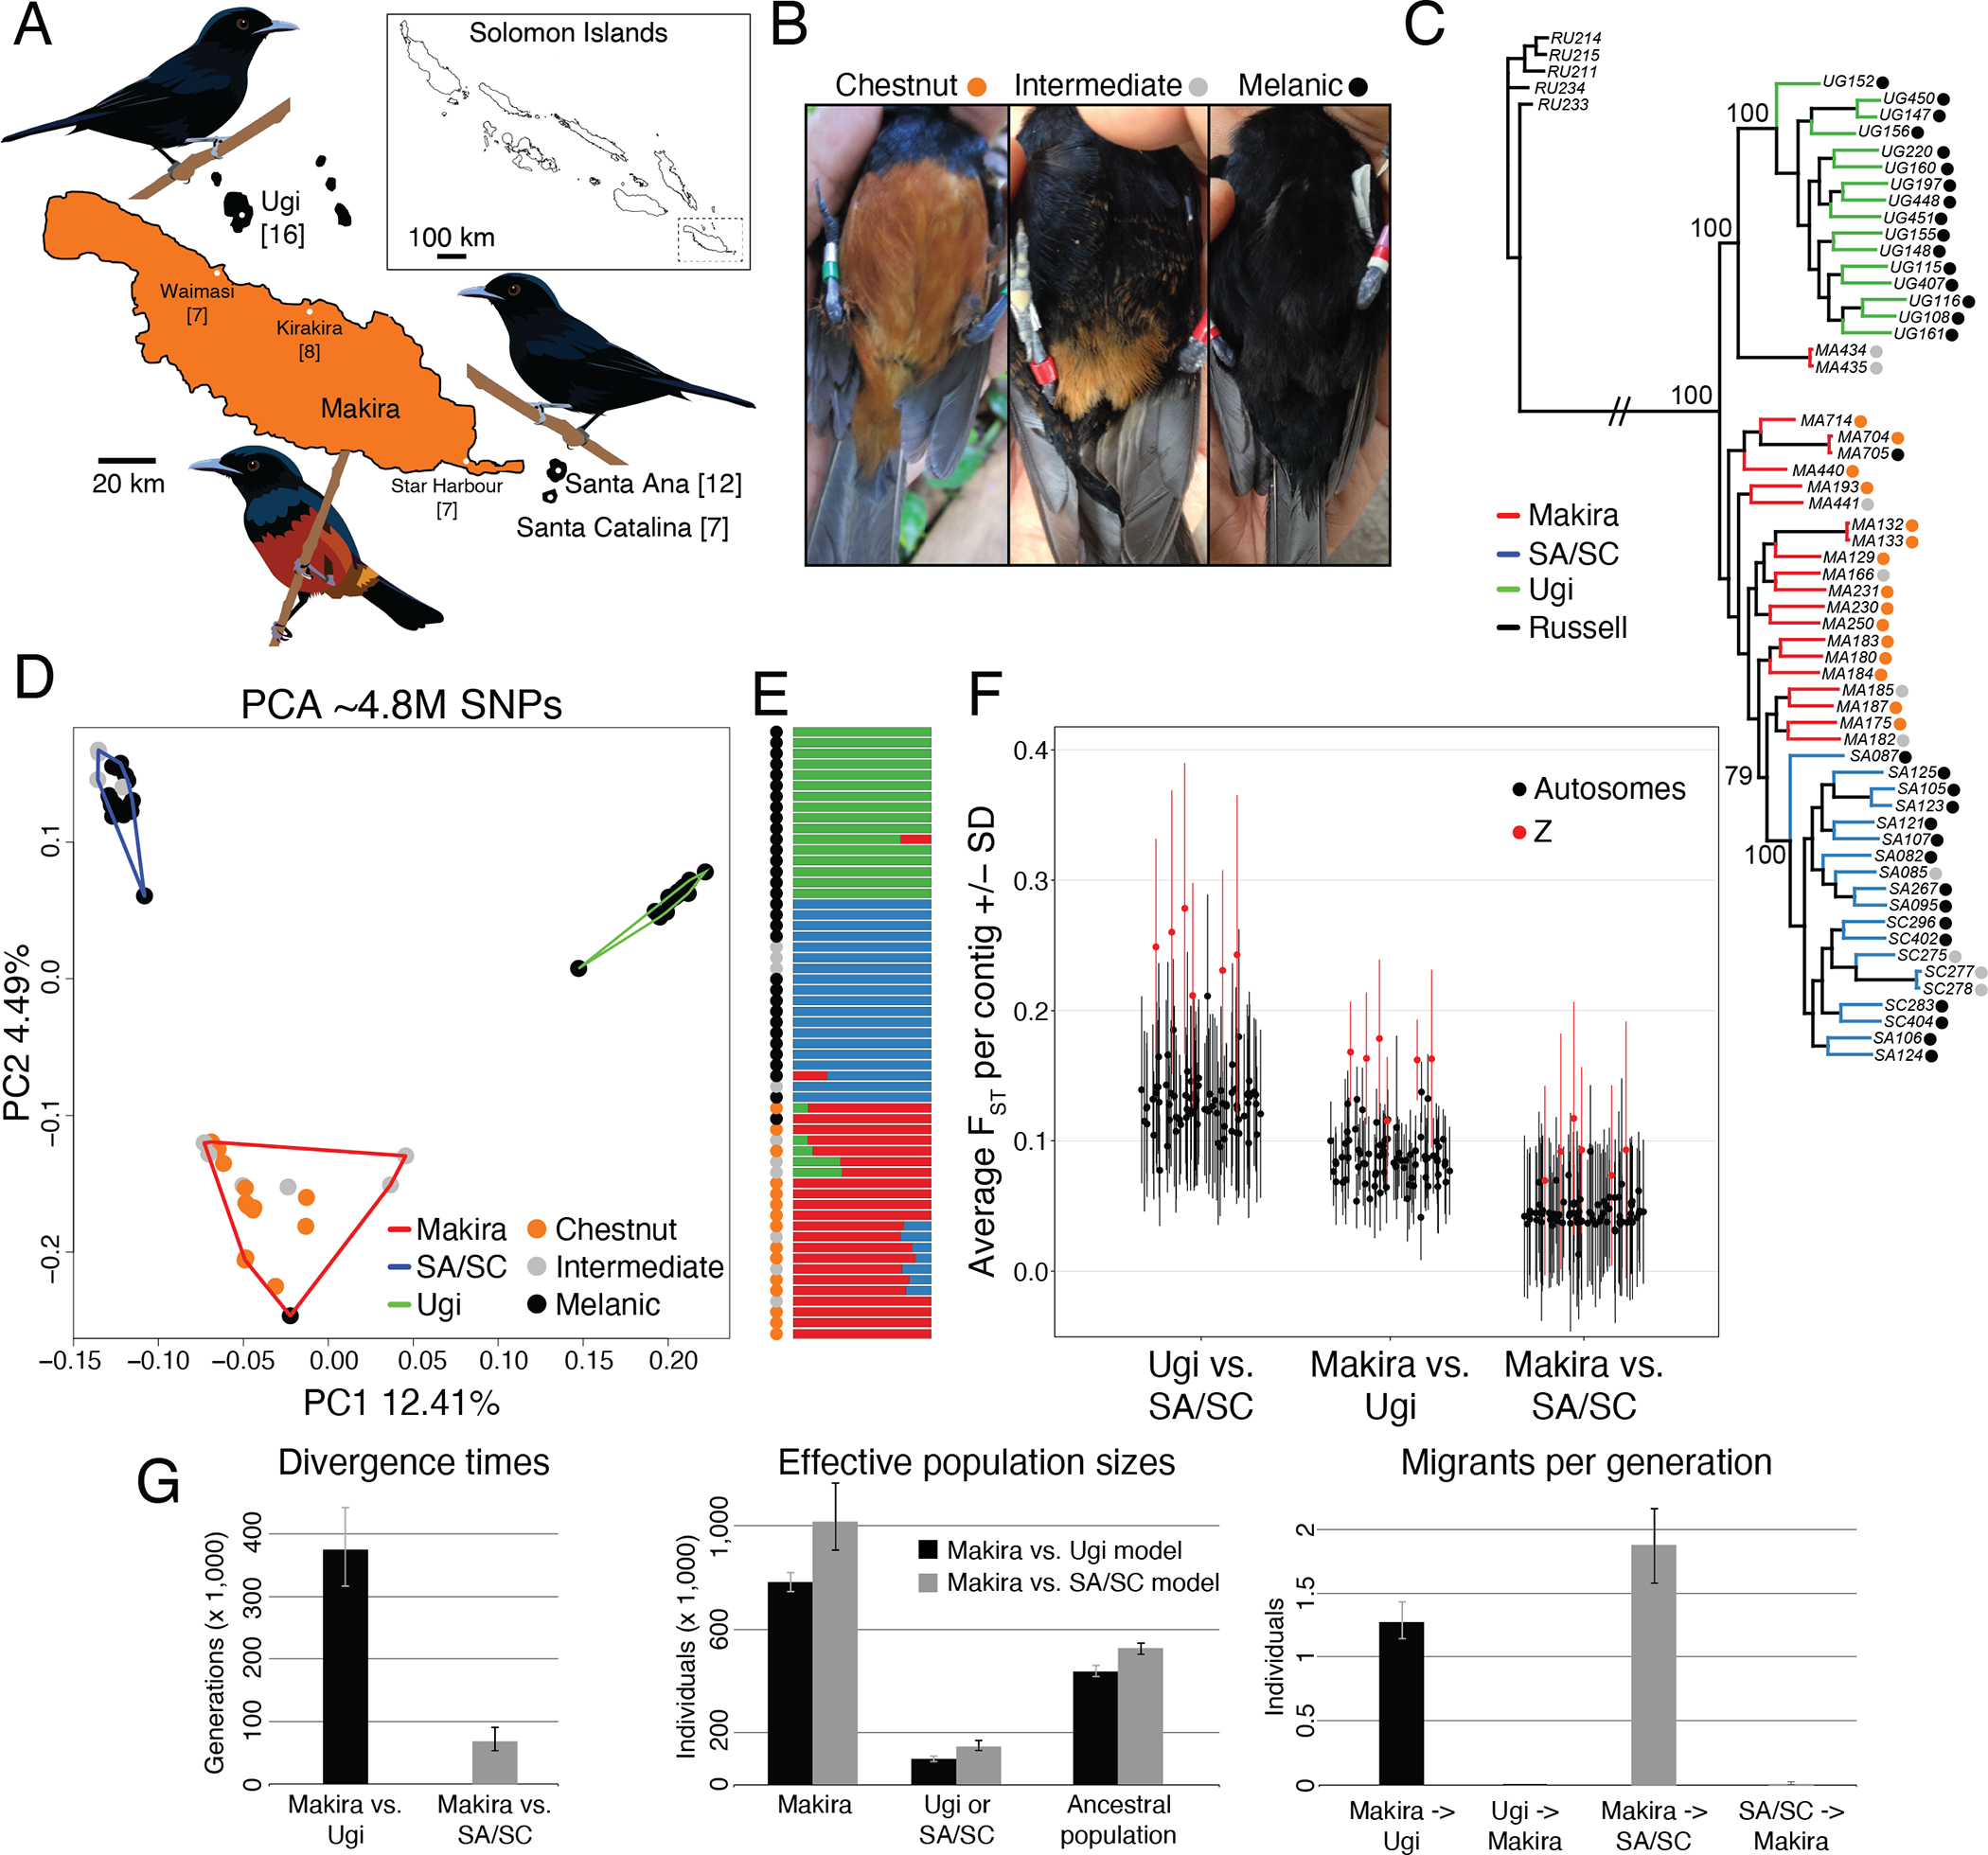
\includegraphics[width=\textwidth]{monarcha_figs/mon_F1.PNG}
    \caption[Genetic differentiation and demography of \textit{M. c. megarhynchus} and \textit{M. c. ugiensis}.]{\textbf{Genetic differentiation and demography of \textit{M. c. megarhynchus} and \textit{M. c. ugiensis}.} \textbf{A.} Study area, sample sizes and predominant phenotype on each island. The map was downloaded and modified from \href{www.diva-gis.org}{www.diva-gis.org}. \textbf{B.} Representative pictures of chestnut-bellied, intermediate and melanic individuals (color key used throughout Chapter \ref{chapter3}). Maximum Likelihood tree (\textbf{C}) and \acs{PCA} (\textbf{D}) indicating the origin and coloration phenotype of each individual. \textbf{E.} Admixture plot showing the proportion of ancestry for each individual belonging to three different genetic clusters. Each cluster is color-coded by the island from which samples originated and the phenotype is shown by color-coded circles on the left of the plot. \textbf{F.} Pairwise $F_{\mathrm{ST}}$ estimates summarized by contig. \textbf{G.} Demographic reconstructions indicating estimates of divergence times, effective population sizes, and migrants per generation.}
    \label{fig:mon-F1}
\end{figure}

Here we generate a reference genome for the Chestnut-bellied Monarch and obtain high coverage whole-genome data for a sample of individuals from Makira and its satellite islands. Our study aims to uncover the molecular targets and evolutionary forces that shape convergent evolution of adaptive traits that can contribute to generating prezygotic reproductive isolation. We use these data to quantify differentiation, reconstruct phylogenetic affinities, and infer the demographic history of these populations. We then use a genome-wide approach to identify variants associated with melanic plumage. Finally, we infer the evolutionary processes that have shaped these phenotypes on each of the satellite islands of Ugi and \ac{SA/SC}, estimate when mutations arose and the timing of these selective events.

\section{Results}

\subsection{Melanic populations are independently derived from a chestnut-bellied ancestor}

\section{Discussion}

\section{Materials and methods}

\section{Supplementary material}
Supporting information is available at \href{https://journals.plos.org/PLOSGENETICS/article?id=10.1371/journal.pgen.1010474#sec017}{\textit{PLoS Genetics} online}. The computer code for this project has been deposited in GitHub repos, \href{https://github.com/CshlSiepelLab/bird_capuchino_analysis}{\texttt{bird\_capuchino\_analysis}} and \href{https://github.com/CshlSiepelLab/arg-selection}{\texttt{arg-selection}}. Genomic data have been archived in GenBank (BioProject ID PRJNA835722).